\documentclass[11pt, a4paper]{article}\usepackage[]{graphicx}\usepackage[]{xcolor}
% maxwidth is the original width if it is less than linewidth
% otherwise use linewidth (to make sure the graphics do not exceed the margin)
\makeatletter
\def\maxwidth{ %
  \ifdim\Gin@nat@width>\linewidth
    \linewidth
  \else
    \Gin@nat@width
  \fi
}
\makeatother

\definecolor{fgcolor}{rgb}{0.345, 0.345, 0.345}
\newcommand{\hlnum}[1]{\textcolor[rgb]{0.686,0.059,0.569}{#1}}%
\newcommand{\hlsng}[1]{\textcolor[rgb]{0.192,0.494,0.8}{#1}}%
\newcommand{\hlcom}[1]{\textcolor[rgb]{0.678,0.584,0.686}{\textit{#1}}}%
\newcommand{\hlopt}[1]{\textcolor[rgb]{0,0,0}{#1}}%
\newcommand{\hldef}[1]{\textcolor[rgb]{0.345,0.345,0.345}{#1}}%
\newcommand{\hlkwa}[1]{\textcolor[rgb]{0.161,0.373,0.58}{\textbf{#1}}}%
\newcommand{\hlkwb}[1]{\textcolor[rgb]{0.69,0.353,0.396}{#1}}%
\newcommand{\hlkwc}[1]{\textcolor[rgb]{0.333,0.667,0.333}{#1}}%
\newcommand{\hlkwd}[1]{\textcolor[rgb]{0.737,0.353,0.396}{\textbf{#1}}}%
\let\hlipl\hlkwb

\usepackage{framed}
\makeatletter
\newenvironment{kframe}{%
 \def\at@end@of@kframe{}%
 \ifinner\ifhmode%
  \def\at@end@of@kframe{\end{minipage}}%
  \begin{minipage}{\columnwidth}%
 \fi\fi%
 \def\FrameCommand##1{\hskip\@totalleftmargin \hskip-\fboxsep
 \colorbox{shadecolor}{##1}\hskip-\fboxsep
     % There is no \\@totalrightmargin, so:
     \hskip-\linewidth \hskip-\@totalleftmargin \hskip\columnwidth}%
 \MakeFramed {\advance\hsize-\width
   \@totalleftmargin\z@ \linewidth\hsize
   \@setminipage}}%
 {\par\unskip\endMakeFramed%
 \at@end@of@kframe}
\makeatother

\definecolor{shadecolor}{rgb}{.97, .97, .97}
\definecolor{messagecolor}{rgb}{0, 0, 0}
\definecolor{warningcolor}{rgb}{1, 0, 1}
\definecolor{errorcolor}{rgb}{1, 0, 0}
\newenvironment{knitrout}{}{} % an empty environment to be redefined in TeX

\usepackage{alltt}

\usepackage[top=1 in, bottom = 1 in, left = 1 in, right = 1 in ]{geometry}

\usepackage{amsmath, amssymb, amsfonts}
\usepackage{enumerate}
\usepackage{array}
\usepackage{multirow}
\usepackage{dingbat}
\usepackage{fontawesome5}
\usepackage{tasks}
\usepackage{bbding}

\title{MSMS - 105}
\author{Ananda Biswas}
\date{}
\IfFileExists{upquote.sty}{\usepackage{upquote}}{}
\begin{document}

\maketitle

\begin{center}
\textbf{Assignment 01}
\end{center}


\OrnamentDiamondSolid \hspace{0.5cm} \textcolor{blue}{\textbf{Task :}} Collect a real data set belongs to your nearby. The sample size must be more than 20 with at least 4 different variables. Give the inference for this data using basic descriptive statistics and EDA approach. \\


\faArrowAltCircleRight[regular] \textcolor{orange}{\textbf{\textit{Data Description}}} : A data-set has been created with help of the information obtained from students of Semester 1 of Statistics and Computing of DST-CIMS, BHU. A brief description of the data-set is as follows : \\

\textcolor{blue}{\textit{\textbf{gender}}} : gender of the student; \\

\textcolor{blue}{\textit{\textbf{home\_state}}} : home state of the student; \\

\textcolor{blue}{\textit{\textbf{CUET\_score}}} : score of the student in CUET PG Statistics 2024; \\

\textcolor{blue}{\textit{\textbf{appeared\_in\_JAM}}} : 1 if the student had appeared in JAM MS 2024, 0 otherwise; \\

\textcolor{blue}{\textit{\textbf{JAM\_score}}} : score of an appearing student in JAM MS 2024; \\

\textcolor{blue}{\textit{\textbf{coaching}}} : 1 if the student had enrolled in any coaching institute for preparation of aforesaid examinations, 0 otherwise; \\

\textcolor{blue}{\textit{\textbf{UG\_CGPA}}} : CGPA of the student in his/her undergraduate program; \\

\textcolor{blue}{\textit{\textbf{UG\_University\_State}}} : state of the university from where the student has completed his/her undergraduate program.



\begin{knitrout}
\definecolor{shadecolor}{rgb}{0.969, 0.969, 0.969}\color{fgcolor}\begin{kframe}
\begin{alltt}
\hlkwd{dim}\hldef{(raw_data)}
\end{alltt}
\begin{verbatim}
## [1] 44  8
\end{verbatim}
\end{kframe}
\end{knitrout}
There are records of 44 students of the 8 variables as mentioned above.

\begin{knitrout}
\definecolor{shadecolor}{rgb}{0.969, 0.969, 0.969}\color{fgcolor}\begin{kframe}
\begin{alltt}
\hlkwd{names}\hldef{(raw_data)}
\end{alltt}
\begin{verbatim}
## [1] "gender"              "home_state"          "CUET_score"         
## [4] "appeared_in_JAM"     "JAM_score"           "coaching"           
## [7] "UG_CGPA"             "UG_university_state"
\end{verbatim}
\end{kframe}
\end{knitrout}

\newpage


Let us have a look how different states are represented by students grouped by gender.




\begin{knitrout}
\definecolor{shadecolor}{rgb}{0.969, 0.969, 0.969}\color{fgcolor}\begin{kframe}
\begin{alltt}
\hldef{home_state_and_gender} \hlopt
  \hlkwd{ggplot}\hldef{(}\hlkwd{aes}\hldef{(}\hlkwc{x} \hldef{=} \hlkwd{fct_infreq}\hldef{(home.state),} \hlkwc{fill} \hldef{= gender))} \hlopt{+}
  \hlkwd{geom_bar}\hldef{(}\hlkwc{position} \hldef{=} \hlsng{"dodge"}\hldef{,} \hlkwc{col} \hldef{=} \hlsng{"black"}\hldef{,} \hlkwc{linewidth} \hldef{=} \hlnum{0.6}\hldef{)} \hlopt{+}
  \hlkwd{labs}\hldef{(}\hlkwc{x} \hldef{=} \hlsng{"Home State"}\hldef{,} \hlkwc{y} \hldef{=} \hlsng{"Count"}\hldef{,}
       \hlkwc{title} \hldef{=} \hlsng{"State Distribution of Students"}\hldef{)} \hlopt{+}
  \hlkwd{theme}\hldef{(}\hlkwc{legend.position} \hldef{=} \hlsng{"top"}\hldef{)}
\end{alltt}
\end{kframe}
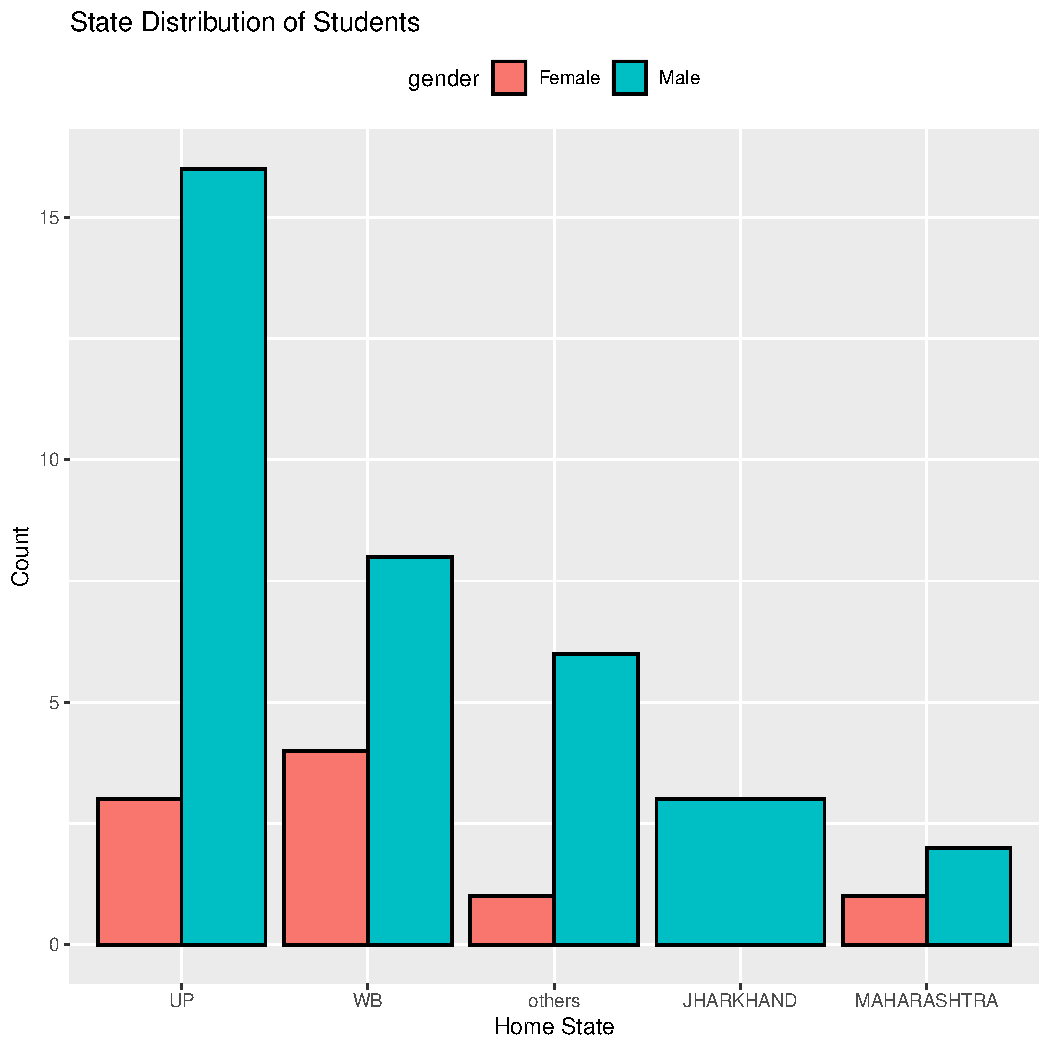
\includegraphics[width=\maxwidth]{figure/unnamed-chunk-7-1} 
\end{knitrout}

\newpage
\begin{knitrout}
\definecolor{shadecolor}{rgb}{0.969, 0.969, 0.969}\color{fgcolor}\begin{kframe}
\begin{alltt}
\hlkwd{table}\hldef{(raw_data}\hlopt{$}\hldef{gender)}
\end{alltt}
\begin{verbatim}
## 
## Female   Male 
##      9     35
\end{verbatim}
\end{kframe}
\end{knitrout}
\smallpencil \hspace{0.5cm} Our data have 9 female students and 35 male students. \\



\leftpointright \textcolor{blue}{\textit{\textbf{CUET\_score}}} \\

Let us plot the values of \textit{\textbf{CUET\_score}} along the real line.





\begin{figure}[!htbp]
\centering

\includegraphics[scale = 0.4]{cuet_score_point_plot.png}
\end{figure}

$\bullet$ \underline{Measure of Central Tendency} : Mean CUET score of the students is 137.6136364. \\

$\bullet$ \underline{Measure of Dispersion} : CUET score has a standard deviation of 18.9088584. \\

$\bullet$ \underline{Quartiles} : The following are the quartiles of CUET score :
\begin{knitrout}
\definecolor{shadecolor}{rgb}{0.969, 0.969, 0.969}\color{fgcolor}\begin{kframe}
\begin{alltt}
\hlkwd{quantile}\hldef{(raw_data}\hlopt{$}\hldef{CUET_score,} \hlkwc{probs} \hldef{=} \hlkwd{c}\hldef{(}\hlnum{0.25}\hldef{,} \hlnum{0.5}\hldef{,} \hlnum{0.75}\hldef{))}
\end{alltt}
\begin{verbatim}
##    25%    50%    75% 
## 124.00 138.00 153.25
\end{verbatim}
\end{kframe}
\end{knitrout}

\leftpointright \textcolor{blue}{\textit{\textbf{JAM\_score}}} \\

Let us plot the values of \textit{\textbf{JAM\_score}} along the real line.

\begin{knitrout}
\definecolor{shadecolor}{rgb}{0.969, 0.969, 0.969}\color{fgcolor}\begin{kframe}
\begin{alltt}
\hldef{df1} \hlkwb{<-} \hldef{raw_data} \hlopt
  \hlkwd{drop_na}\hldef{()}
\end{alltt}
\end{kframe}
\end{knitrout}





\begin{figure}[!htbp]
\centering

\includegraphics[scale = 0.4]{jam_score_point_plot.png}
\end{figure}

$\bullet$ \underline{Measure of Central Tendency} : Mean JAM score of the students is 33.2770588. \\

$\bullet$ \underline{Measure of Dispersion} : JAM score has a standard deviation of 12.3388096. \\

$\bullet$ \underline{Quartiles} : The following are the quartiles of JAM score :
\begin{knitrout}
\definecolor{shadecolor}{rgb}{0.969, 0.969, 0.969}\color{fgcolor}\begin{kframe}
\begin{alltt}
\hlkwd{quantile}\hldef{(df1}\hlopt{$}\hldef{JAM_score,} \hlkwc{probs} \hldef{=} \hlkwd{c}\hldef{(}\hlnum{0.25}\hldef{,} \hlnum{0.5}\hldef{,} \hlnum{0.75}\hldef{))}
\end{alltt}
\begin{verbatim}
##     25%     50%     75% 
## 23.7525 31.1650 40.1875
\end{verbatim}
\end{kframe}
\end{knitrout}

\newpage

\leftpointright \textcolor{blue}{\textit{\textbf{UG\_CGPA}}} \\

Let us plot the values of \textit{\textbf{UG\_CGPA}} along the real line.





\begin{figure}[!htbp]
\centering

\includegraphics[scale = 0.4]{ug_cgpa_point_plot.png}
\end{figure}

$\bullet$ \underline{Measure of Central Tendency} : Mean UG CGPA of the students is 7.8235682. \\

$\bullet$ \underline{Measure of Dispersion} : UG CGPA has a standard deviation of 0.9138116. \\

$\bullet$ \underline{Quartiles} : The following are the quartiles of UG CGPA :
\begin{knitrout}
\definecolor{shadecolor}{rgb}{0.969, 0.969, 0.969}\color{fgcolor}\begin{kframe}
\begin{alltt}
\hlkwd{quantile}\hldef{(raw_data}\hlopt{$}\hldef{UG_CGPA,} \hlkwc{probs} \hldef{=} \hlkwd{c}\hldef{(}\hlnum{0.25}\hldef{,} \hlnum{0.5}\hldef{,} \hlnum{0.75}\hldef{))}
\end{alltt}
\begin{verbatim}
##    25%    50%    75% 
## 7.2000 7.8735 8.4200
\end{verbatim}
\end{kframe}
\end{knitrout}

\smallpencil \hspace{0.5cm} 25\% of the students have UG CGPA more than 8.42. \\

\anchor \hspace{0.2cm} \textbf{Coefficient of Variation}

\begin{knitrout}
\definecolor{shadecolor}{rgb}{0.969, 0.969, 0.969}\color{fgcolor}\begin{kframe}
\begin{alltt}
\hldef{coefficient_of_variation} \hlkwb{<-} \hlkwa{function}\hldef{(}\hlkwc{x}\hldef{,} \hlkwc{na.rm} \hldef{=} \hlnum{FALSE}\hldef{)\{}
  \hlkwd{return}\hldef{(}\hlkwd{sd}\hldef{(x,} \hlkwc{na.rm} \hldef{= na.rm)} \hlopt{/} \hlkwd{mean}\hldef{(x,} \hlkwc{na.rm} \hldef{= na.rm))}
\hldef{\}}
\end{alltt}
\end{kframe}
\end{knitrout}

\begin{knitrout}
\definecolor{shadecolor}{rgb}{0.969, 0.969, 0.969}\color{fgcolor}\begin{kframe}
\begin{alltt}
\hlkwd{coefficient_of_variation}\hldef{(raw_data}\hlopt{$}\hldef{CUET_score)}
\end{alltt}
\begin{verbatim}
## [1] 0.1374054
\end{verbatim}
\end{kframe}
\end{knitrout}

\begin{knitrout}
\definecolor{shadecolor}{rgb}{0.969, 0.969, 0.969}\color{fgcolor}\begin{kframe}
\begin{alltt}
\hlkwd{coefficient_of_variation}\hldef{(raw_data}\hlopt{$}\hldef{JAM_score,} \hlkwc{na.rm} \hldef{=} \hlnum{TRUE}\hldef{)}
\end{alltt}
\begin{verbatim}
## [1] 0.3707903
\end{verbatim}
\end{kframe}
\end{knitrout}

\begin{knitrout}
\definecolor{shadecolor}{rgb}{0.969, 0.969, 0.969}\color{fgcolor}\begin{kframe}
\begin{alltt}
\hlkwd{coefficient_of_variation}\hldef{(raw_data}\hlopt{$}\hldef{UG_CGPA)}
\end{alltt}
\begin{verbatim}
## [1] 0.1168024
\end{verbatim}
\end{kframe}
\end{knitrout}

\smallpencil \hspace{0.5cm} So \textcolor{blue}{\textit{\textbf{UG\_CGPA}}} has minimum variability. \\

\anchor \hspace{0.2cm} \textbf{Correlations}

\begin{knitrout}
\definecolor{shadecolor}{rgb}{0.969, 0.969, 0.969}\color{fgcolor}\begin{kframe}
\begin{alltt}
\hlkwd{cor}\hldef{(df1}\hlopt{$}\hldef{CUET_score, df1}\hlopt{$}\hldef{JAM_score)}
\end{alltt}
\begin{verbatim}
## [1] 0.4714785
\end{verbatim}
\end{kframe}
\end{knitrout}

\begin{knitrout}\footnotesize
\definecolor{shadecolor}{rgb}{0.969, 0.969, 0.969}\color{fgcolor}\begin{kframe}
\begin{alltt}
\hlkwd{cor}\hldef{(raw_data}\hlopt{$}\hldef{CUET_score, raw_data}\hlopt{$}\hldef{UG_CGPA)}
\end{alltt}
\begin{verbatim}
## [1] 0.2304253
\end{verbatim}
\end{kframe}
\end{knitrout}

\begin{knitrout}\footnotesize
\definecolor{shadecolor}{rgb}{0.969, 0.969, 0.969}\color{fgcolor}\begin{kframe}
\begin{alltt}
\hlkwd{cor}\hldef{(df1}\hlopt{$}\hldef{JAM_score, df1}\hlopt{$}\hldef{UG_CGPA)}
\end{alltt}
\begin{verbatim}
## [1] 0.07943115
\end{verbatim}
\end{kframe}
\end{knitrout}

\smallpencil \hspace{0.5cm} \textcolor{blue}{\textit{\textbf{UG\_CGPA}}} and \textcolor{blue}{\textit{\textbf{JAM\_score}}} have moderate correlation. \\


\leftpointright \hspace{0.2cm} \textbf{Method of Preparation of the Students}



\begin{knitrout}\footnotesize
\definecolor{shadecolor}{rgb}{0.969, 0.969, 0.969}\color{fgcolor}\begin{kframe}
\begin{alltt}
\hldef{raw_data} \hlopt
  \hlkwd{ggplot}\hldef{(}\hlkwd{aes}\hldef{(}\hlkwc{x} \hldef{=} \hlkwd{fct_infreq}\hldef{(coaching)))} \hlopt{+}
  \hlkwd{geom_bar}\hldef{(}\hlkwc{fill} \hldef{=} \hlsng{"#fb9c48"}\hldef{,} \hlkwc{width} \hldef{=} \hlnum{0.5}\hldef{,} \hlkwc{col} \hldef{=} \hlsng{"black"}\hldef{,} \hlkwc{linewidth} \hldef{=} \hlnum{1}\hldef{)} \hlopt{+}
  \hlkwd{labs}\hldef{(}\hlkwc{x} \hldef{=} \hlsng{"Enrolled in a Coaching"}\hldef{,} \hlkwc{y} \hldef{=} \hlsng{"Count"}\hldef{,} \hlkwc{title} \hldef{=} \hlsng{"Coaching Enrollment"}\hldef{)}
\end{alltt}
\end{kframe}
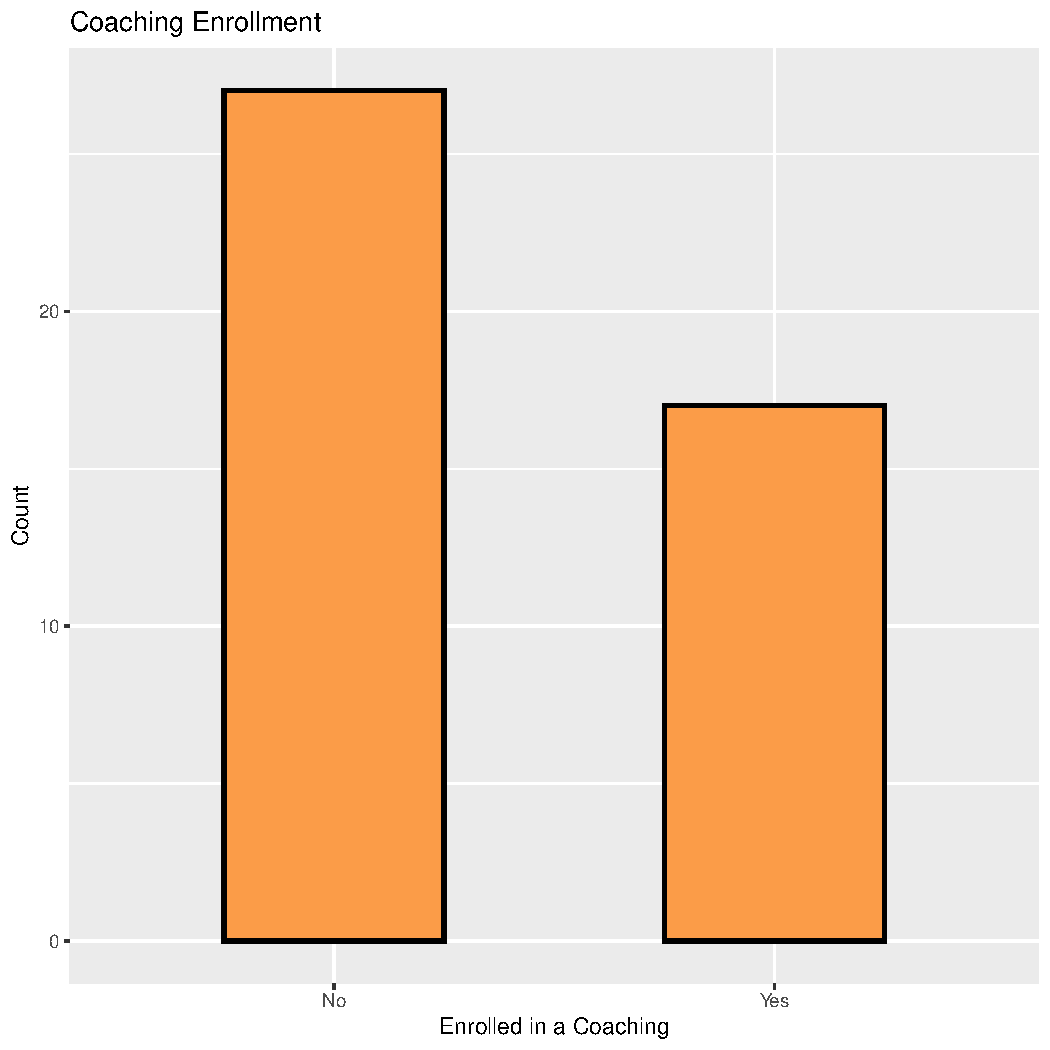
\includegraphics[width=\maxwidth]{figure/unnamed-chunk-27-1} 
\end{knitrout}

\smallpencil \hspace{0.5cm} So greater number of students prepared for competitive exam by self-study only. \\

\newpage

\leftpointright \hspace{0.2cm} \textbf{CUET Score for Two Methods of Preparation}

\begin{knitrout}
\definecolor{shadecolor}{rgb}{0.969, 0.969, 0.969}\color{fgcolor}\begin{kframe}
\begin{alltt}
\hldef{raw_data} \hlopt
  \hlkwd{ggplot}\hldef{(}\hlkwd{aes}\hldef{(}\hlkwc{x} \hldef{=} \hlkwd{as.factor}\hldef{(coaching),} \hlkwc{y} \hldef{= CUET_score))} \hlopt{+}
  \hlkwd{stat_boxplot}\hldef{(}\hlkwc{geom} \hldef{=} \hlsng{"errorbar"}\hldef{,} \hlkwc{linewidth} \hldef{=} \hlnum{1}\hldef{)} \hlopt{+}
  \hlkwd{geom_boxplot}\hldef{(}\hlkwc{fill} \hldef{=} \hlsng{"#b548fb"}\hldef{,} \hlkwc{linewidth} \hldef{=} \hlnum{0.7}\hldef{)} \hlopt{+}
  \hlkwd{labs}\hldef{(}\hlkwc{x} \hldef{=} \hlsng{"Coaching"}\hldef{,} \hlkwc{y} \hldef{=} \hlsng{"CUET Score"}\hldef{,} \hlkwc{title} \hldef{=} \hlsng{"CUET Score vs Coaching Enrollment"}\hldef{)}
\end{alltt}
\end{kframe}
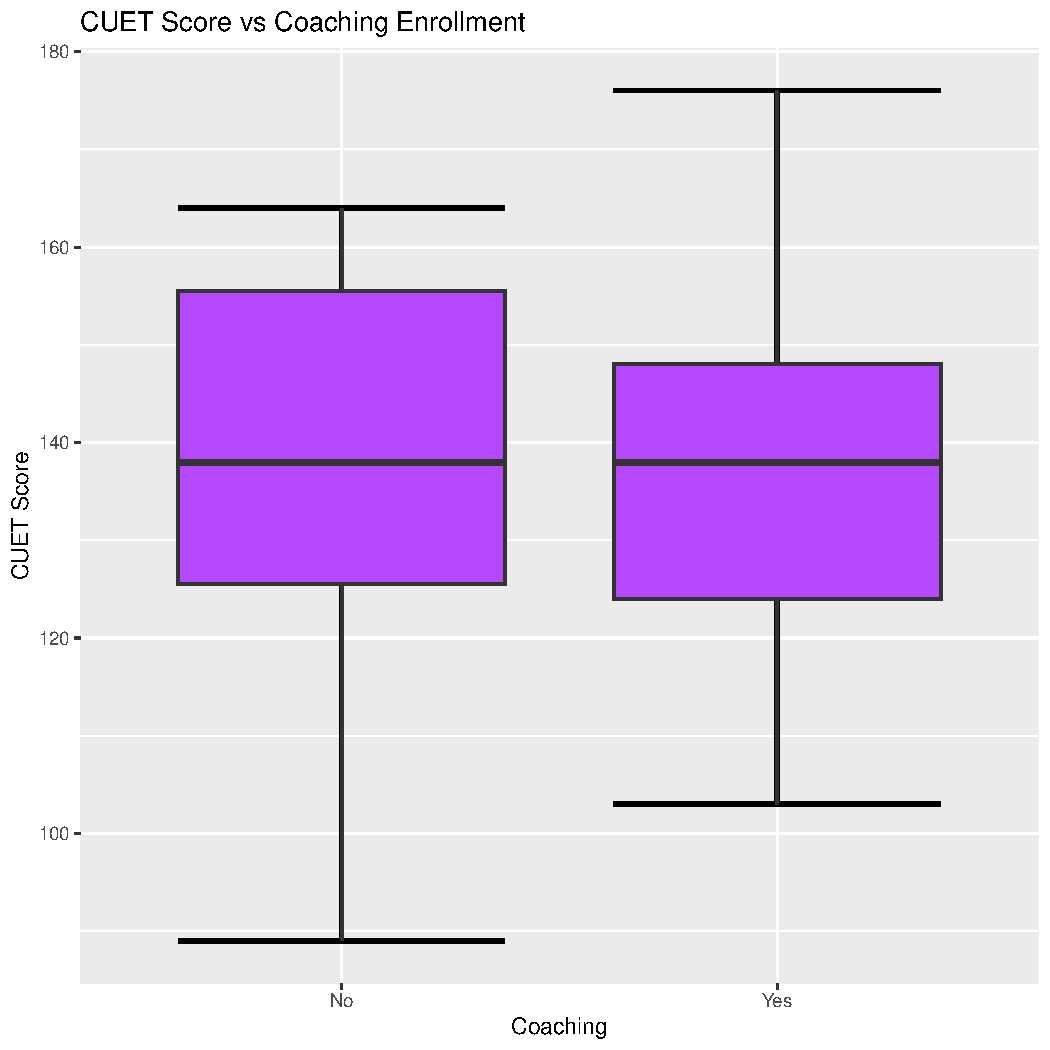
\includegraphics[width=\maxwidth]{figure/unnamed-chunk-28-1} 
\end{knitrout}

\smallpencil \hspace{0.5cm} Median score of students who enrolled in a coaching institute and the ones who didn't are almost the same.

\newpage

\leftpointright \hspace{0.2cm} \textbf{UG CGPA for Male and Female Students}

\begin{knitrout}
\definecolor{shadecolor}{rgb}{0.969, 0.969, 0.969}\color{fgcolor}\begin{kframe}
\begin{alltt}
\hldef{raw_data} \hlopt
  \hlkwd{ggplot}\hldef{(}\hlkwd{aes}\hldef{(}\hlkwc{x} \hldef{= gender,} \hlkwc{y} \hldef{= UG_CGPA))} \hlopt{+}
  \hlkwd{stat_boxplot}\hldef{(}\hlkwc{geom} \hldef{=} \hlsng{"errorbar"}\hldef{,} \hlkwc{linewidth} \hldef{=} \hlnum{1}\hldef{)} \hlopt{+}
  \hlkwd{geom_boxplot}\hldef{(}\hlkwc{fill} \hldef{=} \hlsng{"#fb48a2"}\hldef{,} \hlkwc{linewidth} \hldef{=} \hlnum{0.7}\hldef{)} \hlopt{+}
  \hlkwd{labs}\hldef{(}\hlkwc{x} \hldef{=} \hlsng{"Gender"}\hldef{,} \hlkwc{y} \hldef{=} \hlsng{"UG CGPA"}\hldef{)}
\end{alltt}
\end{kframe}
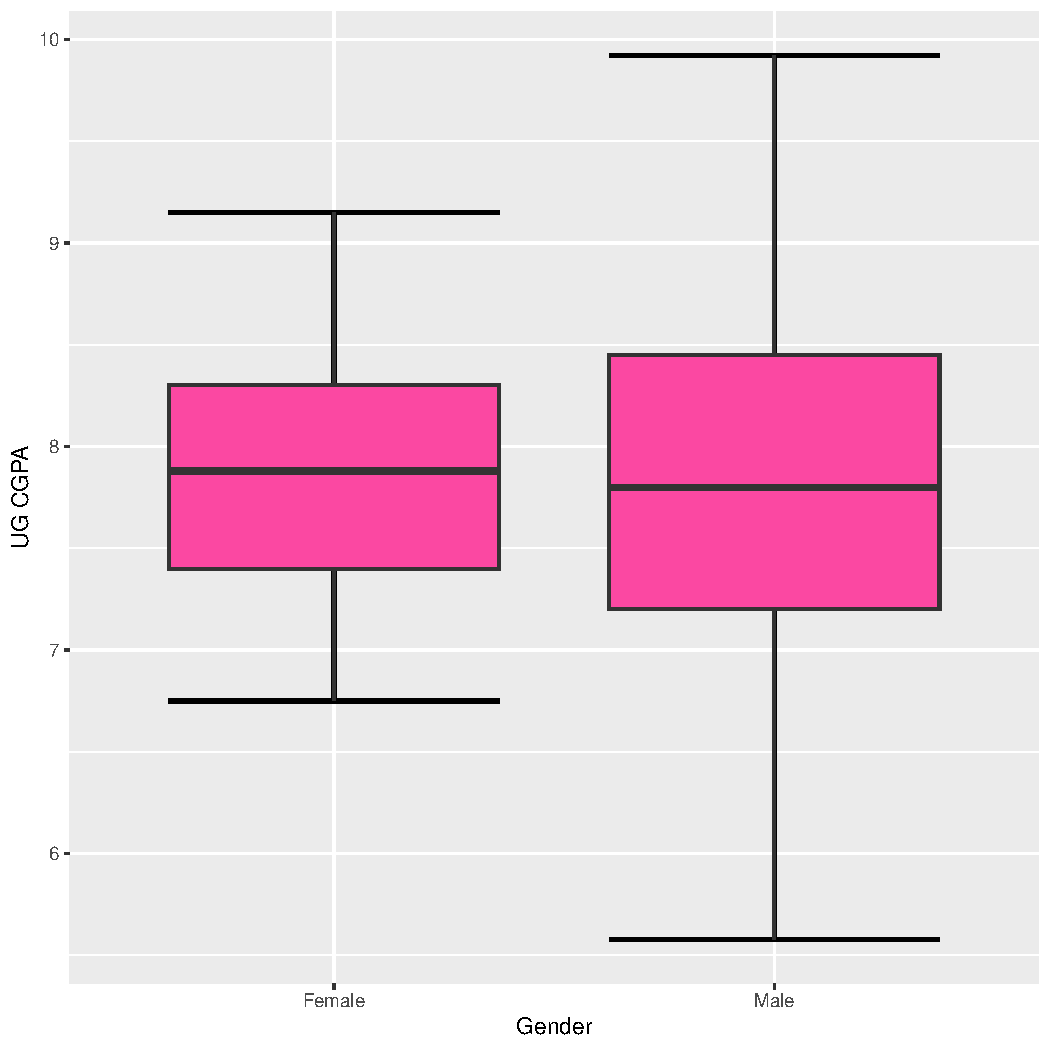
\includegraphics[width=\maxwidth]{figure/unnamed-chunk-29-1} 
\end{knitrout}

\smallpencil \hspace{0.5cm} Average UG CGPA of female students is slightly higher than that of male students. Also the CGPAs of male students have greater dispersion.

\newpage

\leftpointright \hspace{0.2cm} \textbf{Frequency Distribution of CUET Score}

\begin{knitrout}
\definecolor{shadecolor}{rgb}{0.969, 0.969, 0.969}\color{fgcolor}\begin{kframe}
\begin{alltt}
\hldef{raw_data} \hlopt
  \hlkwd{ggplot}\hldef{(}\hlkwd{aes}\hldef{(}\hlkwc{x} \hldef{= CUET_score))} \hlopt{+}
  \hlkwd{geom_histogram}\hldef{(}\hlkwc{fill} \hldef{=} \hlsng{"#0FD8F0"}\hldef{,} \hlkwc{bins} \hldef{=} \hlnum{10}\hldef{,} \hlkwc{col} \hldef{=} \hlsng{"black"}\hldef{,} \hlkwc{linewidth} \hldef{=} \hlnum{1}\hldef{)} \hlopt{+}
  \hlkwd{labs}\hldef{(}\hlkwc{x} \hldef{=} \hlsng{"CUET Score"}\hldef{,} \hlkwc{y} \hldef{=} \hlsng{"Frequency Density"}\hldef{,} \hlkwc{title} \hldef{=} \hlsng{"Distribution of CUET Score"}\hldef{)}
\end{alltt}
\end{kframe}
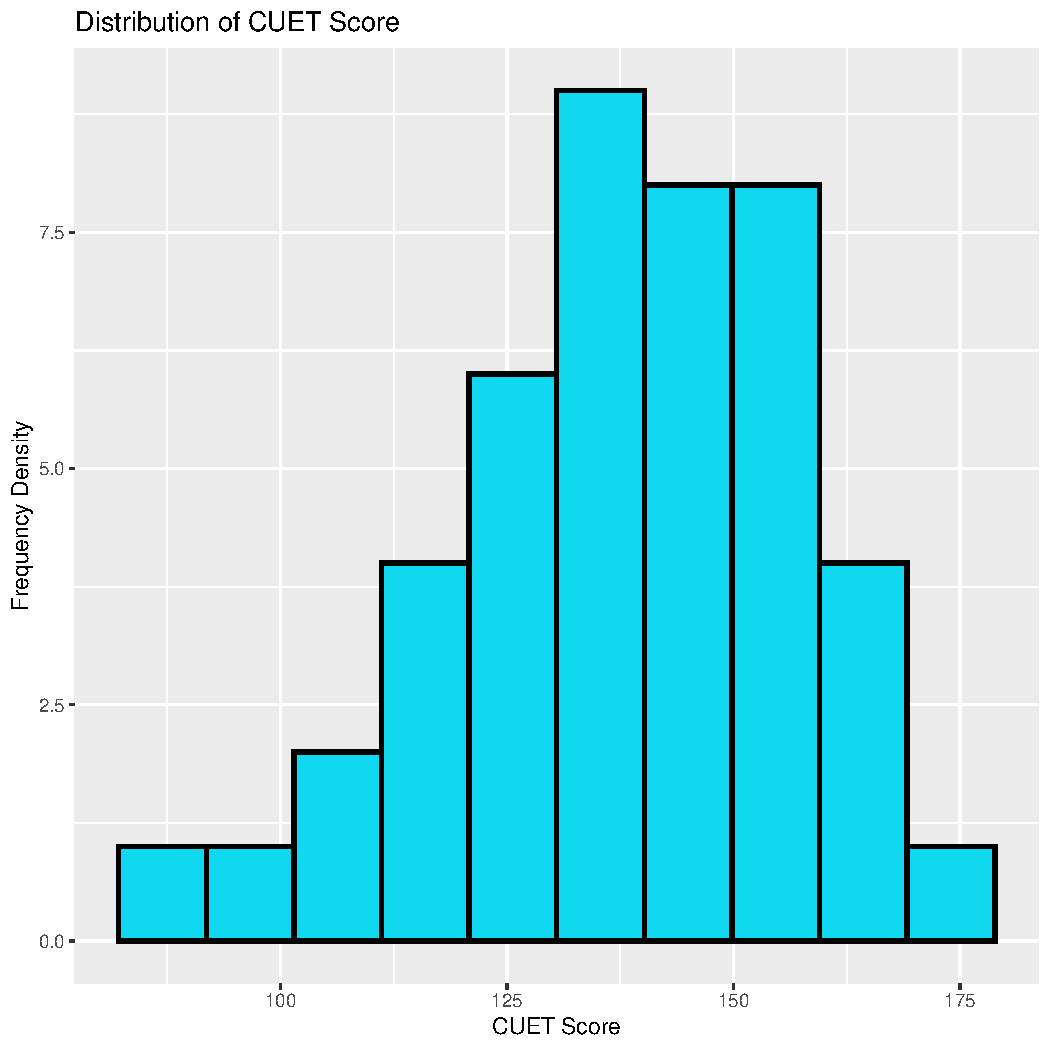
\includegraphics[width=\maxwidth]{figure/unnamed-chunk-30-1} 
\end{knitrout}

\newpage

\leftpointright \hspace{0.2cm} \textbf{CUET Score for Students of Different States}



\begin{knitrout}
\definecolor{shadecolor}{rgb}{0.969, 0.969, 0.969}\color{fgcolor}\begin{kframe}
\begin{alltt}
\hldef{score_univ_state} \hlopt
  \hlkwd{ggplot}\hldef{(}\hlkwd{aes}\hldef{(}\hlkwc{x} \hldef{= univ.state,} \hlkwc{y} \hldef{= score))} \hlopt{+}
  \hlkwd{stat_boxplot}\hldef{(}\hlkwc{geom} \hldef{=} \hlsng{"errorbar"}\hldef{,} \hlkwc{linewidth} \hldef{=} \hlnum{0.7}\hldef{)} \hlopt{+}
  \hlkwd{geom_boxplot}\hldef{(}\hlkwc{fill} \hldef{=} \hlsng{"#3bfa89"}\hldef{,} \hlkwc{linewidth} \hldef{=} \hlnum{0.5}\hldef{)} \hlopt{+}
  \hlkwd{labs}\hldef{(}\hlkwc{x} \hldef{=} \hlsng{"UG University State"}\hldef{,} \hlkwc{y} \hldef{=} \hlsng{"CUET Score"}\hldef{,}
       \hlkwc{title} \hldef{=} \hlsng{"CUET Score ~ UG University State"}\hldef{)}
\end{alltt}
\end{kframe}
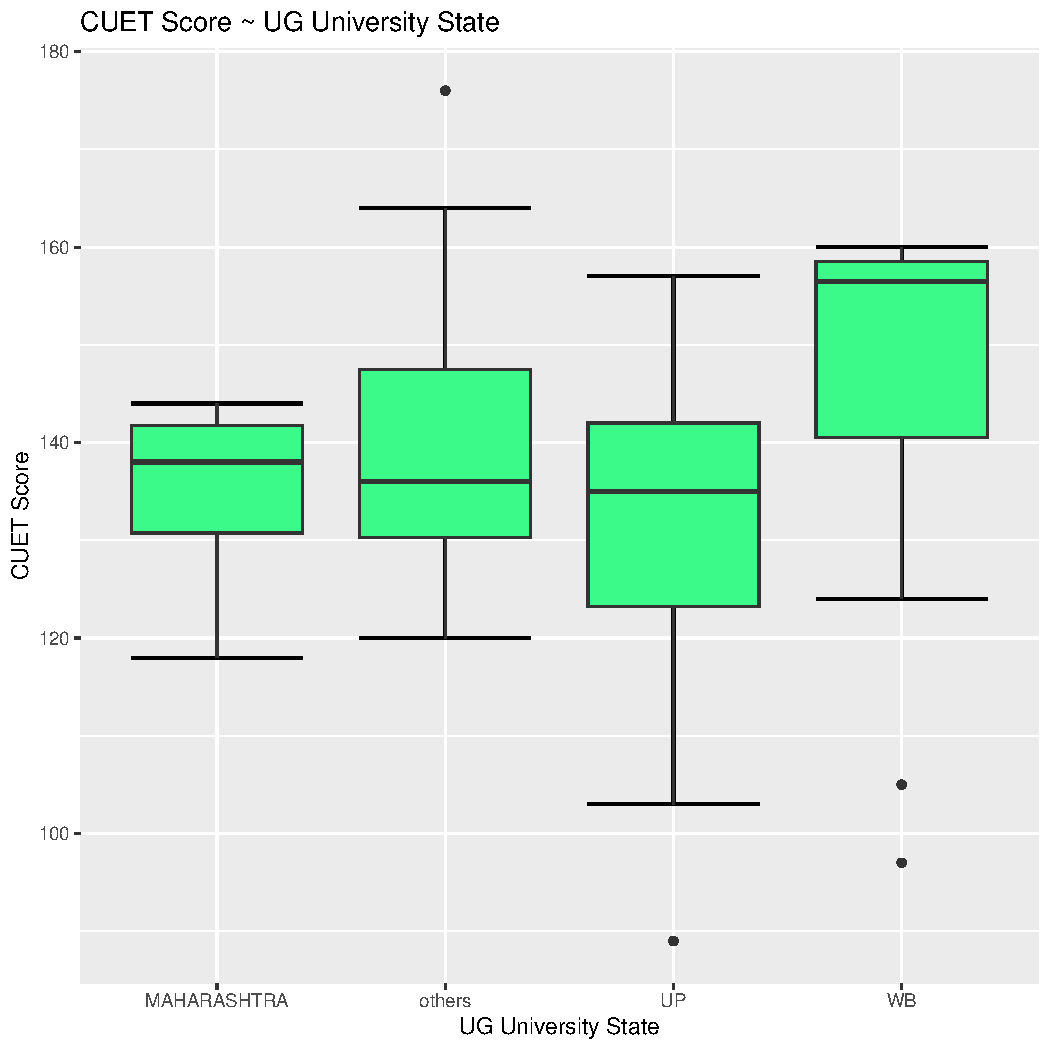
\includegraphics[width=\maxwidth]{figure/unnamed-chunk-32-1} 
\end{knitrout}

\smallpencil \hspace{0.5cm} Clearly, students from the Universities of West Bengal have better CUET Scores than rest of the students.

\end{document}
